\documentclass{article}
\usepackage[utf8]{inputenc}
\usepackage[papersize={8.5in,11in},margin=0.8in]{geometry}
\usepackage{adjustbox}
\usepackage{xcolor}
\usepackage{color, colortbl}
\usepackage{graphicx}
\usepackage{pgfplots}
\usepackage{amsmath}
\pgfplotsset{compat=1.17}

\title{MATH 505 Assignment 4}
\author{John Caruthers}
\date\today

\begin{document}
\maketitle

\noindent
Let $A=\{0,1,2,3,4\}$, $B=\{-2,-1,0,1,2\}$, $C=\{4,5,6,7,8,9\}$, and $D=\{a,b,c\}$.  Create a graph of the following functions with specified domains and codomains.  Then decide if it is one-to-one or onto.

\noindent
{\color{blue} The x axis is the domain and the y axis is the codomain (range).}

\begin{itemize}
    \item[1.] $f:A \to B$, where $f=\{(0,0),(1,-2),(2,2),(3,1),(4,0)\}$ {\color{blue} Neither one-to-one or onto.}
    
    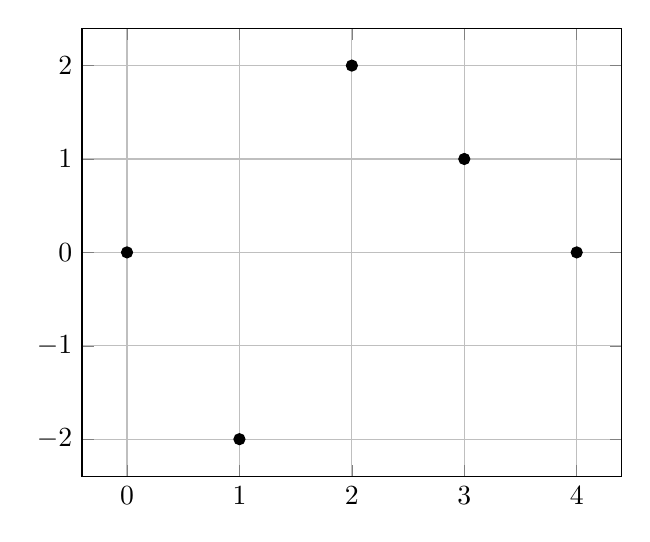
\begin{tikzpicture}
    \begin{axis}[ymajorgrids=true,xmajorgrids=true]
    \addplot[only marks]
        coordinates {
        (0,0)(1,-2)(2,2)(3,1)(4,0)
        };
    \end{axis}
    \end{tikzpicture}
    
    \item[2.] $g:A \to B$, where $g(x)=x-2$
    {\color{blue} Both one-to-one and onto.}
    
    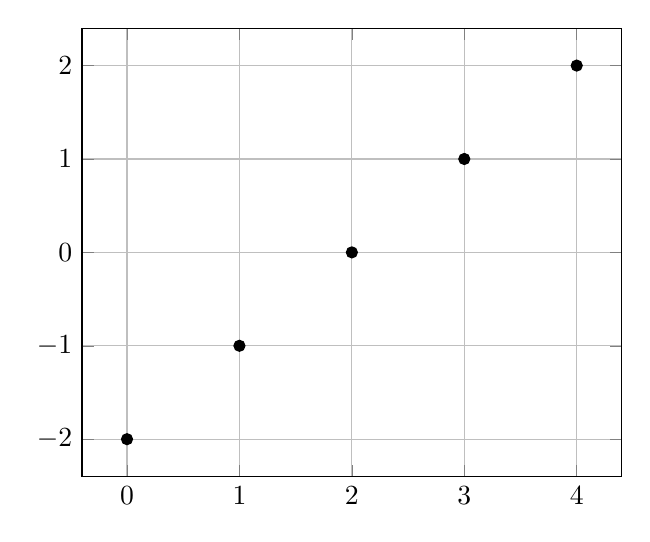
\begin{tikzpicture}
    \begin{axis}[ymajorgrids=true,xmajorgrids=true]
    \addplot[only marks]
        coordinates {
        (0,-2)(1,-1)(2,0)(3,1)(4,2)
        };
    \end{axis}
    \end{tikzpicture}
    
    \newpage
    
    \item[3.] $h:B \to A$, where $h=\{(-2,4),(-1,1),(0,0),(1,1),(2,4)\}${\color{blue} Neither one-to-one or onto.}
    
    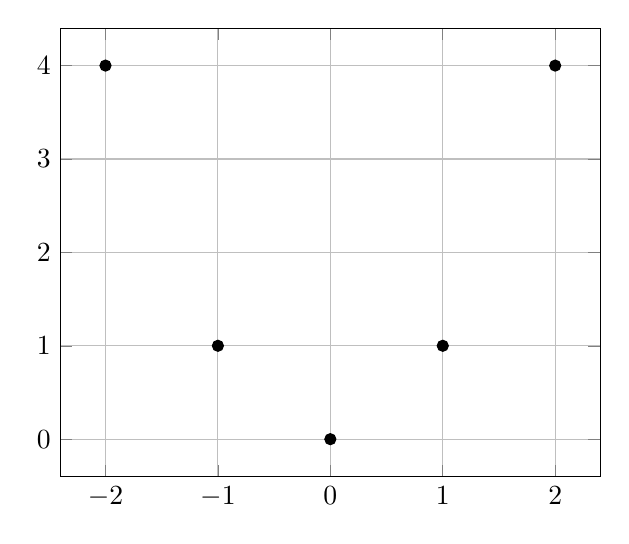
\begin{tikzpicture}
    \begin{axis}[ymajorgrids=true,xmajorgrids=true]
    \addplot[only marks]
        coordinates {
        (-2,4)(-1,1)(0,0)(1,1)(2,4)
        };
    \end{axis}
    \end{tikzpicture} 
    
    \item[4.] $k:A \to C$, where $k(x)=x+4$ {\color{blue} Only one-to-one.}
    
    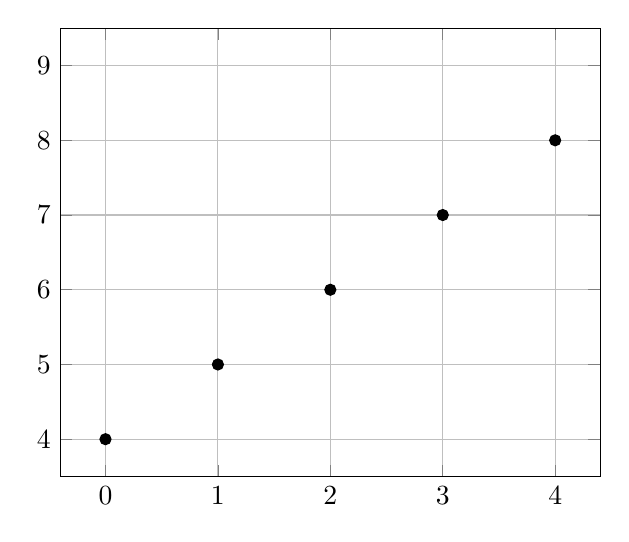
\begin{tikzpicture}
    \begin{axis}[
        ytick={4,5,6,7,8,9},
        ymajorgrids=true,xmajorgrids=true]
    \addplot[only marks]
        coordinates {
        (0,4)(1,5)(2,6)(3,7)(4,8)
        };
    \addplot[]
        coordinates {(4,9)};
    \end{axis}
    \end{tikzpicture}    
    
    \item[5.] $m:A \to D$, where $m=\{(0,b),(1,a),(2,c),(3,a),(4,c)\}$ {\color{blue} Only onto.}
    
    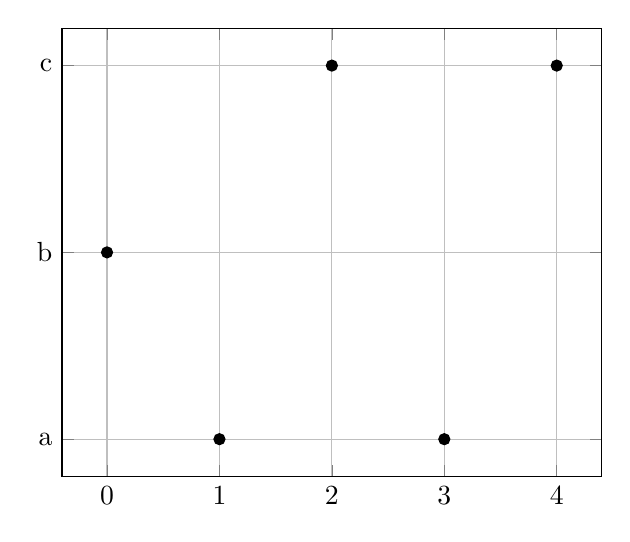
\begin{tikzpicture}
    \begin{axis}[
        ytick={a,b,c},
        symbolic y coords={a,b,c},
        ymajorgrids=true,xmajorgrids=true]
    \addplot[only marks]
        coordinates {
        (0,b)(1,a)(2,c)(3,a)(4,c)
        };
    \end{axis}
    \end{tikzpicture} 
    
    \newpage
    
    \item[6.] $n:D \to A$, where $n=\{(a,1),(b,2),(c,3)\}$     {\color{blue} Only one-to-one.}
    
    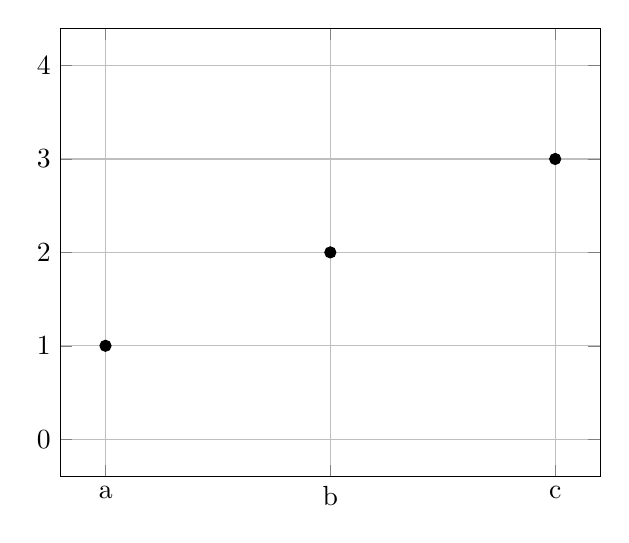
\begin{tikzpicture}
    \begin{axis}[
        xtick={a,b,c},
        ytick={0,1,2,3,4},
        symbolic x coords={a,b,c},
        ymajorgrids=true,xmajorgrids=true]
    \addplot[only marks]
        coordinates {
        (a,1)(b,2)(c,3)
        };
    \addplot[only marks, mark size=0pt]
        coordinates {(a,0)(c,4)};
    \end{axis}
    \end{tikzpicture}     
    
    \item[7.] $p:B \to C$, where $p(x)=9-x^2$ {\color{blue} Neither one-to-one or onto.}
    
    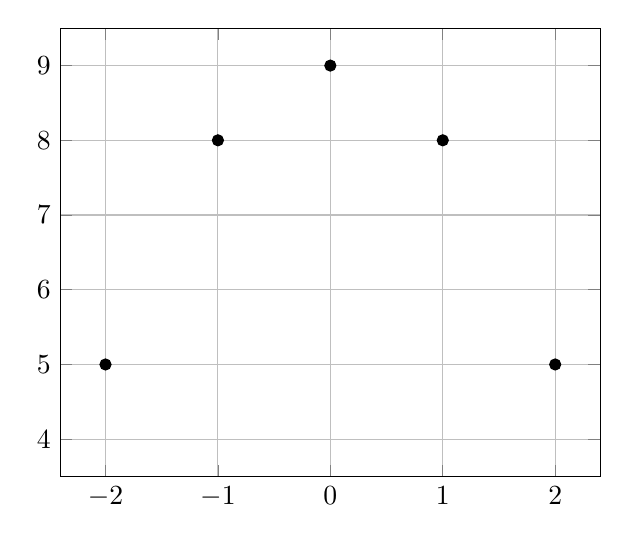
\begin{tikzpicture}
    \begin{axis}[
        ytick={4,5,6,7,8,9},
        ymajorgrids=true,xmajorgrids=true]
    \addplot[only marks]
        coordinates {
        (-2,5)(-1,8)(0,9)(1,8)(2,5)
        };
    \addplot[]
        coordinates {(-2,4)};
    \end{axis}
    \end{tikzpicture}
    
\end{itemize}

\noindent
Consider the cardinality of the domain $X$ and codomain $Y$ for $f:X \to Y$.  Recall, the cardinality is the number of elements of a set $A$, and is written $n(A)$.  Use your answers above to guide you. 

\begin{itemize}
    \item[8.] If $f$ is one-to-one, what can you say about the $n(X)$ compared to $n(Y)$?
    
    {\color{blue} If $f$ is one-to-one, then $n(X) \leq n(Y)$.}
    
    \item[9.] If $f$ is onto, what can you say about the $n(X)$ compared to the $n(Y)$?
    
    {\color{blue} If $f$ is onto, then $n(X) \geq n(Y)$.}
    
    \item[10.] If $f$ is one-to-one and onto, what can you say about the $n(X)$ compared to $n(Y)$?
    
    {\color{blue} If $f$ is both one-to-one and onto, then $n(X)=n(Y)$.}
\end{itemize}

\noindent
The following questions are about sequences.

\begin{itemize}
    \item[11.] Let $a_n=4n-1$. Write the first 7 terms in the sequence. 
    
    {\color{blue} $3,7,11,15,19,23,27,...$}
    
    \item[12.] Is the sequence in $\#11$ arithmetic?  If so, what is $d$, the common difference?  If not, why? 
    
    {\color{blue} The above sequence in arithmetic, $d=4$.}
    
    \item[13.] What are the next 3 terms in the following arithmetic sequence: $12, 7, 2, -3, ...$
    
    {\color{blue} $-8,-13,-18,...$}
    
    \item[14.] Pretend in $\#13$ that the sequence was not necessarily arithmetic, give an alternative answer.
    
    {\color{blue} $\#13$ gives a linear relationship, therefore we can write a linear equation: $y=-4x+16$}
    
    \item[15.] Provide a general formula for your answer in $\#13$.
    
    {\color{blue} $a_n=12-4(n-1)$}
    
    \item[16.] If $b_2=6$ and  $b_5=27$, give a general formula for $b_n$.
    
    {\color{blue} I am assuming this is an arithmetic sequence.  To solve for $b_n$, the initial value ($a_n$) and $d$ must be found.  A system of equations can be formed using the general formula: $b_n=b_1+d(n-1)$. We use this system of equations to solve for $b_1$ and $d$.  Once we have these variables, then a general formula can be written.}
    
    \begin{align}
        n&=2: b_1+d(2-1)=6\\
        n&=5: b_1+d(5-1)=27
    \end{align}
    
    Take eq(1), solve for $b_1$.
    
    \begin{align}
        &b_1+d(2-1)=6\nonumber\\
        &b_1+d=6\nonumber\\
        &b_1=6-d
    \end{align}
    
    Plug $b_1$ into eq(2), solve for $d$.
    
    \begin{align}
        (6-d)+d(5-1)&=27\nonumber\\
        6-d+4d&=27\nonumber\\
        4d-d&=27-6\nonumber\\
        3d&=21\nonumber\\
        d&=7\nonumber
    \end{align}
    
    Plug $d$ into eq(3), solve for $b_1$.
    
    \begin{align}
        b_1&=6-7\nonumber\\
        b_1&=-1\nonumber
    \end{align}
    
    {\color{blue} $b_1=-1$ and $d=7$, therefore the general formula for an arithmetic sequence is: $b_n=-1+7(n-1)$}
\end{itemize}

\end{document}
